\documentclass{beamer}

\usepackage[utf8]{inputenc}
\usepackage{graphicx}
\graphicspath{ {img/} }
\usetheme{Berlin}
\usecolortheme{Crane}

\title[Learning Linux]{Linux: The Command Line}
\author{Jacob Beal}
\date{\today}
\begin{document}
\frame{\titlepage}
\begin{frame}
    \frametitle{Why use the command-line?}
    \begin{itemize}
        \item<1-> More Powerful
        \item<2-> Faster
        \item<3-> Not all programs have graphical interfaces
        \item<4-> Street-Cred
    \end{itemize}
\end{frame}
\begin{frame}
    \frametitle{Quick tip for people on Laptops}
    \begin{block}{Windows}
    Download PuTTY \url{http://www.chiark.greenend.org.uk/~sgtatham/putty/download.html}
    \text<3->{If you are on OS X}
    \end{block}
    \begin{block}{OS X}
    Open a terminal and use ssh.
    \text<3->{If you are on OS X}
    \end{block}
\end{frame}
\begin{frame}
    \frametitle{SSH into Lab computers: OS X}
\begin{semiverbatim}
    ssh \textit{username}@greta-pt.ecs.vuw.ac.nz
\end{semiverbatim}
\end{frame}
\begin{frame}
    \frametitle{SSH into Lab computers: Windows}
    Open up the \verbatim|putty.exe| that you downloaded earlier
    \begin{center}
        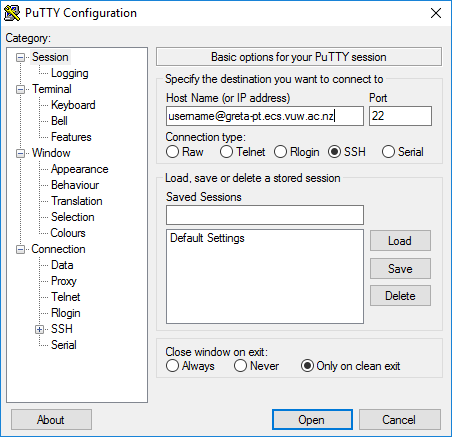
\includegraphics[width=0.4\textwidth]{putty}
    \end{center}
    Then type in your password etc\ldots to get into the \textit{shell} of the
    University computers
\end{frame}
\begin{frame}
    \frametitle{How to start?}
    So, you want to learn how do we start?
\end{frame}
\end{document}
